\section*{Vlastní vstup}
Zadávání vlastního kakura je velmi jednoduché. 
Zavoláte \haskellline/kakuro <vlastni vstup>/, 
kde $<$vlastni vstup$>$ je sekvence [(x,y,z),.....] obalená v hranatých závorkách.
Kakuro se zadává ve čtvercové mřížce, tedy strana čtverce je rovna delší straně kakura.
Nyní se podívame co znamená trojice:
\subsection*{x}
První hodnota trojice je číslo od -2 do 9, kde:\\
-2 je blok, prázdná buňka bez možnosti vyplnění\\
-1 je pomocná buňka, kde je zobrazena suma v řádku a sloupci\\
0 je nevyplněná buňka\\
1 - 9 je buňka vyplněná

\subsection*{y}
Druhá hodnota trojice je suma na řádku v pomocné buňce.
Má hodnoty 0-45.\\
0 je pro jiné buňky než pomocné\\
1 - 45 je suma na řádku v pomocné buňce

\subsection*{z}
Třetí hodnota z trojice je totéž co druhá hodnota, akorát neznačí sumu v řádku, ale v sloupci.

\subsection*{Příklad}
Chceme vypočítat následující kakuro:\\
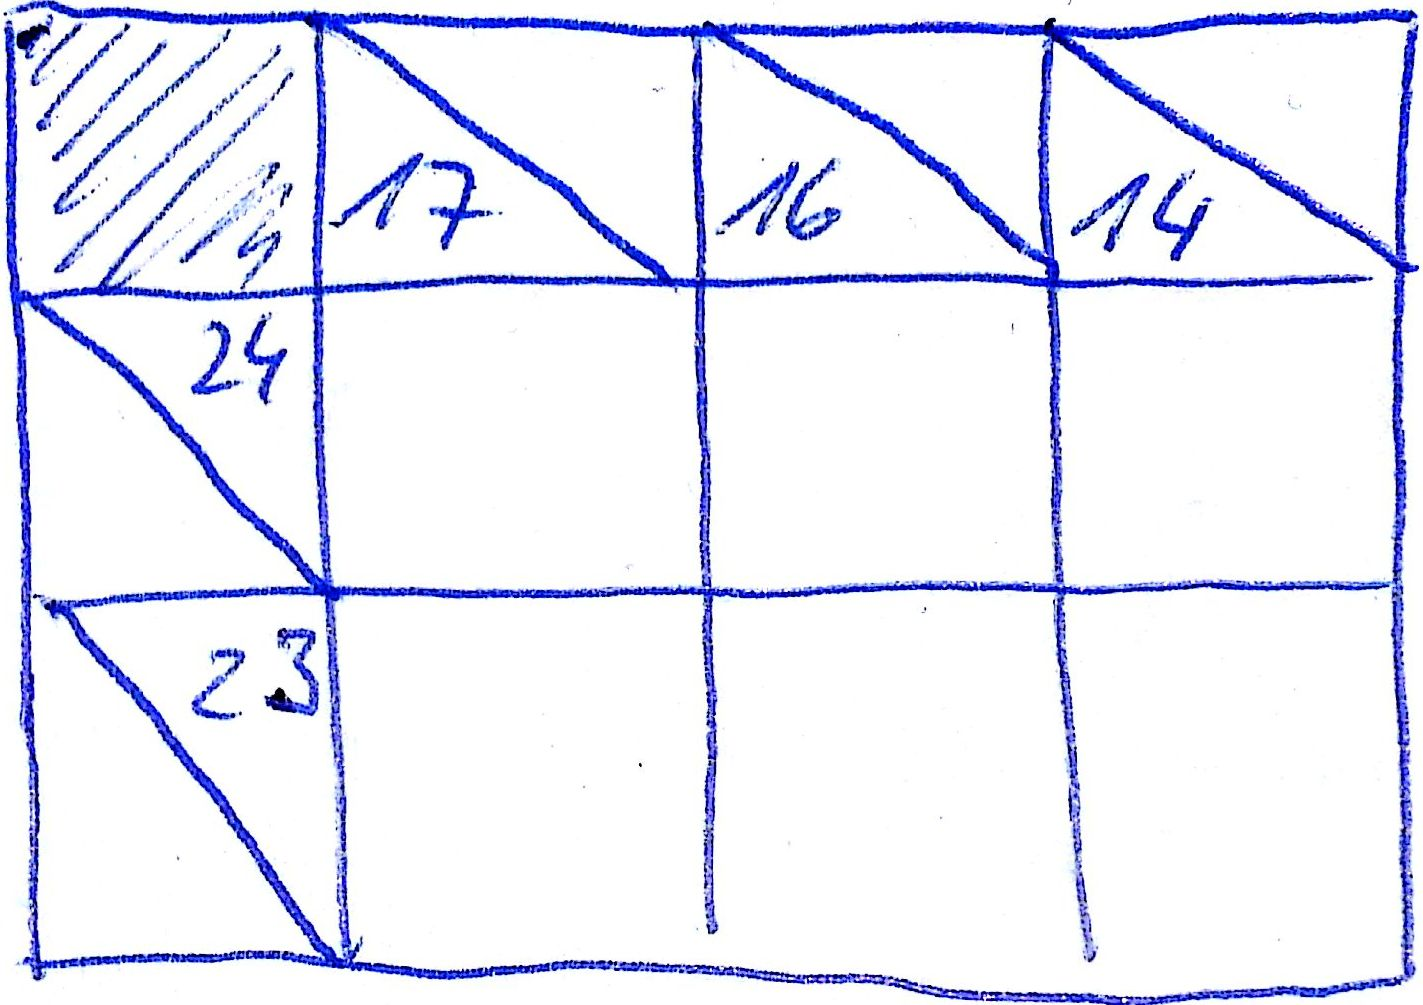
\includegraphics[width=0.75\textwidth]{kakurofrom.jpg}\\
Musíme si ho nejprve převést na čtverec:\\
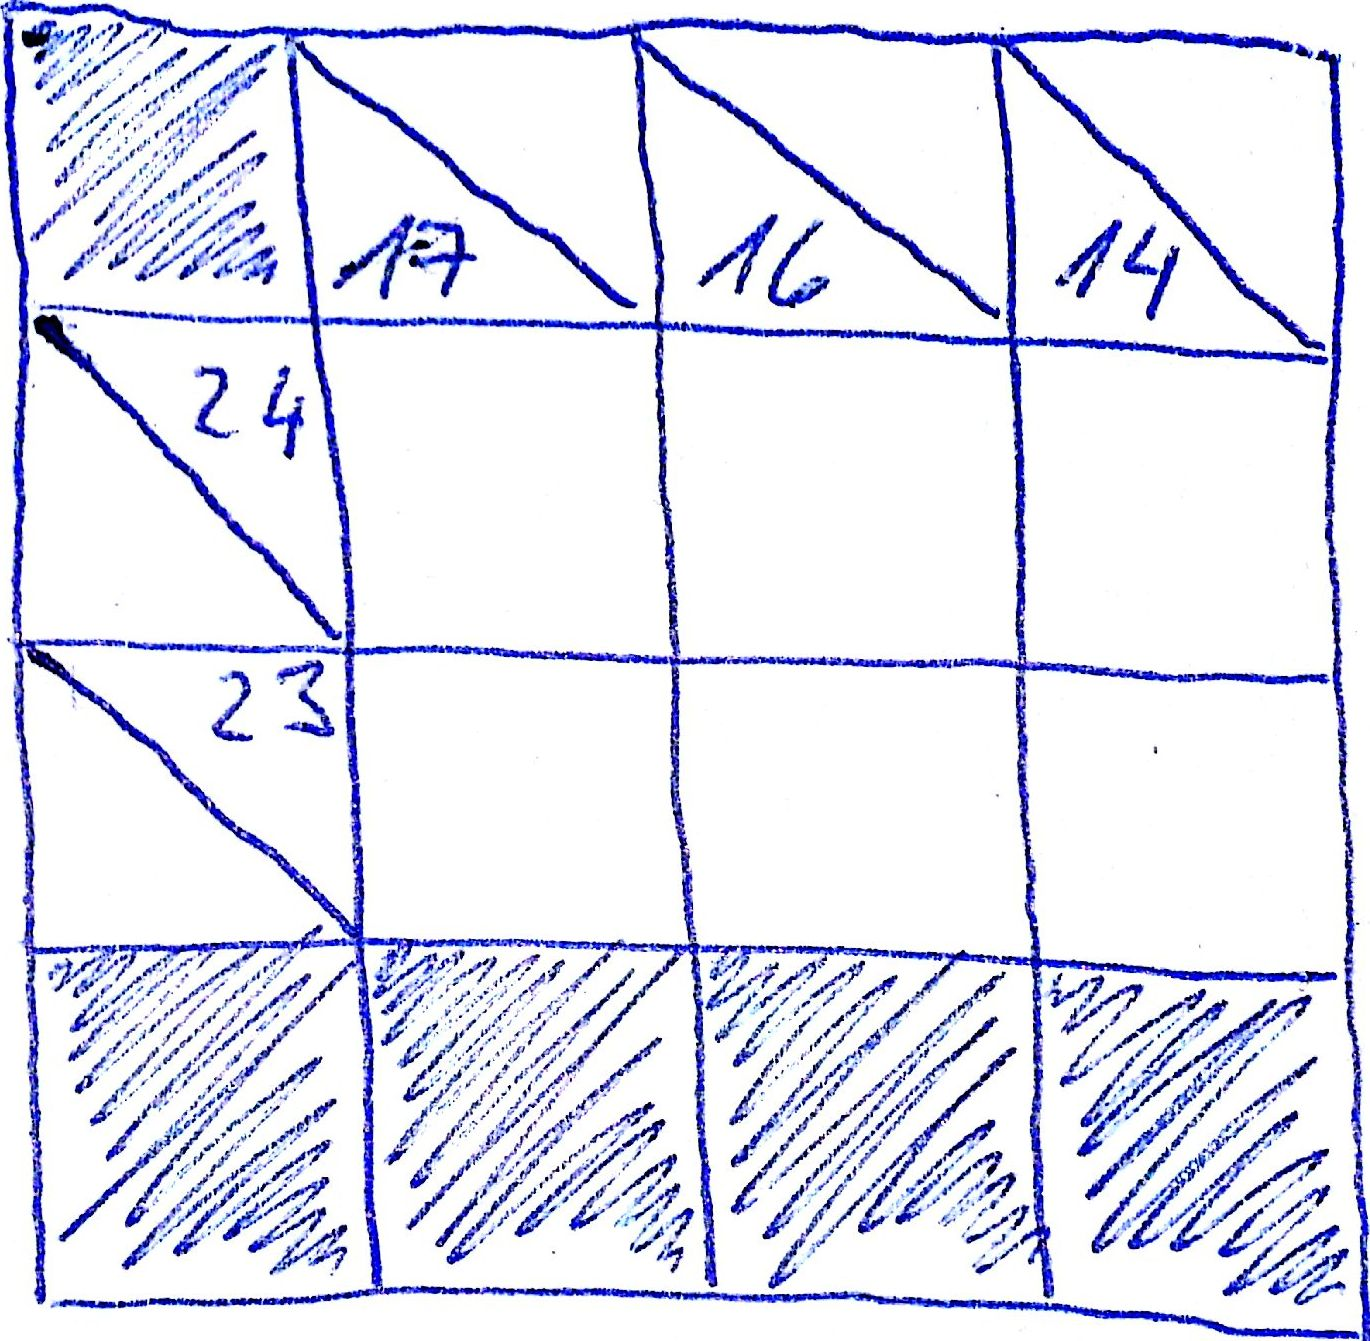
\includegraphics[width=0.75\textwidth]{kakuroto.jpg}\\
A nyní zadáme do programu:
\haskell/kakuro [(-2,0,0), (-1,0,17), (-1,0,16), (-1,0,14), (-1,24,0), (0,0,0), (0,0,0), (0,0,0), (-1,23,0), (0,0,0), (0,0,0), (0,0,0), (-2,0,0), (-2,0,0), (-2,0,0), (-2,0,0)]/

